\FloatBarrier
\begin{figure}[!h]
\centering
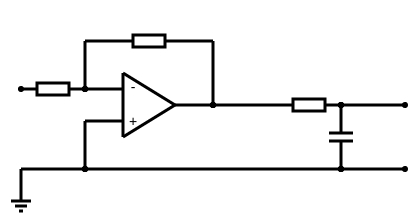
\includegraphics[scale=0.75]{../Grafiken/Ersatzschaltbild.jpg}
\caption{Ersatzschaltbild eines realen Operationsverstärkers 
	in dem dieser durch einen idealen Operationsverstärker und einen 
	nachgeschalteten Tiefpass ersetzt wird. Der Tiefpass beschreibt dabei 
	interne Widerstände und Kapazitäten des realen Operationsverstärkers.
	\label{fig:ersatzschaltbild}}
\end{figure}
\FloatBarrier